\documentclass{beamer}
\usepackage[T1]{fontenc}
\usepackage[utf8]{inputenc}
\usepackage{lmodern} 
\usepackage[portuguese]{babel}
\usepackage{graphicx}			%para imagens
\usepackage{epstopdf} 			%resolve problemas eps-pdf
\usepackage{fancyhdr}			% para o cabeçalho bonito
\usepackage{caption}				%para legendas
\usepackage{placeins} 			%controlar o lugar dos floats
\usepackage{hyperref}
\usepackage{listings}
\usepackage{color}
\usepackage{xcolor}

\lstset{language=Java,
    basicstyle=\ttfamily,
    keywordstyle=\bfseries,
    showstringspaces=false,
    morekeywords={MidiSystem, Soundbank, Synthesizer}
}
\defbeamertemplate*{title page}{customized}[1][]
{
  \usebeamerfont{title}\inserttitle\par
  \usebeamerfont{subtitle}\usebeamercolor[fg]{subtitle}\insertsubtitle\par
  \bigskip
 %% \usebeamerfont{author}\insertauthor\par
  \usebeamerfont{institute}\insertinstitute\par
  \usebeamerfont{date}\insertdate\par
  \usebeamercolor[fg]{titlegraphic}\inserttitlegraphic
}

%DEFINE TEMA BEAMER A SER UTILIZADO
\usetheme{Warsaw}
%DEFINIÇÃO DE TÍTULO, AUTORES .....
\title[Introdução a Computação Sônica]{ ICS - Trabalho II \\ Síntese Aditiva}
%\title[pequeno título que vai no bottom da página]{título grande}%
\author{Juarez A.S.F. 11/0032829}
\institute{Universidade de Brasília}
\date{\today}

\begin{document}


\begin{frame}
        \titlepage
\end{frame}

\AtBeginSection[]
{
%%página com layout da sessão ao início de cada sessão
 \begin{frame}<beamer>
   \tableofcontents[currentsection,currentsubsection]
 \end{frame}
}

\begin{frame}{Requisitos}
	\frametitle{Requisitos}
    \begin{itemize}
	\item Desenvolver uma interface gráfica em Java que implemente três instrumentos aditivos 
	e seja capaz de tocar melodias e notas com ele. A interface deve possuir operações de:
	\begin{itemize}
	 \item Música
	 \item Nota
	 \end{itemize}
    \end{itemize}
\end{frame}

\section{Classes Desenvolvidas}
\subsection{Dispositivo RAN}
\begin{frame}[fragile]
	\frametitle{RAN}
Classe desenvolvida para gerar a envoltória aleatória.	
	\begin{itemize}
		\item extends Envoltoria
		\item entradas controláveis: 
		\begin{itemize}
			\item f\_ran: define o número de amostras aleatórias geradas no intervalo
			\item a: define a amplitude da envoltória gerada. Isto é, os números aleatórios vão de -A até +A
		\end{itemize}
		\item fórmula utilizada para gerar números entre -A e +A :
		\begin{tiny}	\begin{lstlisting}
				float random = 2f*A*((float)Math.random()) - A;		    				
		\end{lstlisting} \end{tiny}	
		
		\item possui método de visualização gerado com o pacote \textbf{jmathtool}					\item Toda vez que um dos dois parâmetros acima é atualizado, uma nova envoltória
		é gerada. Pode-se também gerar uma nova envoltória a qualquer momento.
	\end{itemize}
\end{frame}

\begin{frame}
 \frametitle{Dispositivo RAN}
 \begin{figure}
  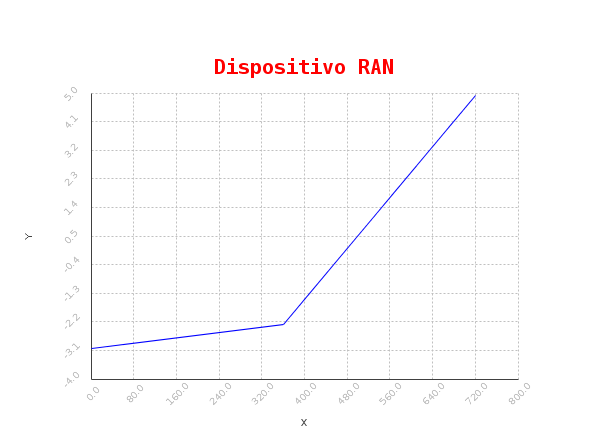
\includegraphics[scale=0.4]{./images/RAN_F_2.png}
  \caption{Dispositivo RAN, f\_ran = 2, A = 10}
   \end{figure}
\end{frame}
   \begin{frame}
 \begin{figure}
  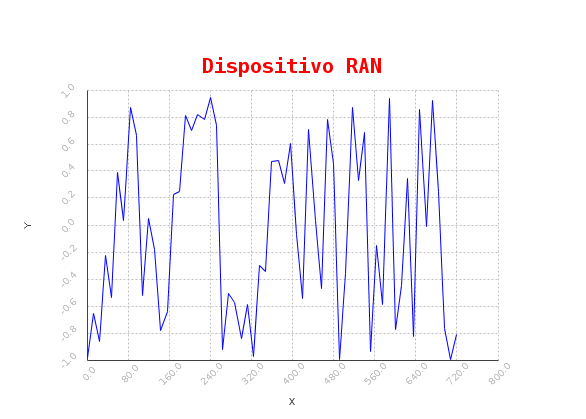
\includegraphics[scale=0.4]{./images/RAN_F_60.png}
  \caption{Dispositivo RAN, f\_ran = 60, A = 1}
 \end{figure} 

\end{frame}


\section{Interface Gráfica em JAVA}

\subsection{Componentes Utilizados}
\begin{frame}
	\frametitle{Componentes}
Alguns componentes utilizados na interface:	
	\begin{itemize}
		\item \textbf{ImageIcon, Icon e JButton} para botões
		\item \textbf{JSlider} para entrada/saída de informações de tempo
		\item \textbf{JLabel e JTable} para informações textuais
		\item \textbf{JMenu, JMenuItem e JMenuBar} para menu
		\item \textbf{JFileChooser} para navegar e carregar arquivo 
		\item \textbf{JTimer} para controlar tempo com que o JSlider é atualizado
	\end{itemize}
\end{frame}

\subsection{Layout}
\begin{frame}
  \frametitle{Composição de Layouts}

\end{frame}




\section{Problemas Encontrados}



\end{document}
